\documentclass[]{IEEEtran}
% some very useful LaTeX packages include:
%\usepackage{cite}      
\usepackage{graphicx}   
\usepackage{subfigure} 
\usepackage{url}       
\usepackage{amsmath}    
\usepackage{caption2}
% Your document starts here!
\begin{document}

% Define document title and author
	\title{Weekly Report}
	\author{Adviser: Prof. Yang Wen \\Student: Cheng Wensheng\\ Period: 2018.10.7-10.13
	}
	\markboth{Visual Information Processing Group}{}
	\maketitle

% Write abstract here
\begin{abstract}
	This week I mainly put my effort on writing project application and reading the paper about multi-scale context semantic segmentation.
\end{abstract}

% Each section begins with a \section{title} command
\section{Paper reading}
	% \PARstart{}{} creates a tall first letter for this first paragraph
	\PARstart{T}{he} paper's title is \emph{Multi-scale context intertwining for semantic segmentation}. In this paper, they propose a novel scheme for aggregating features from different scales, which they refer to as Multi-Scale Context Intertwining (MSCI). In summary, the following points show their main contributions:
	\begin{itemize}
		\item They present a multi-scale context intertwining (MSCI) architecture, where the context information can be propagated along different dimensions. The first dimension is along the vertical deep hierarchy: their context intertwining scheme has connections to exchange the multi-scale context information between
		the adjacent feature maps. The connection is bidirectional with two different long short-term memory (LSTM) chains that intertwines feature maps of different resolution in a sequence of stages. By training the LSTM units, the bidirectional
		connections learn to produce more powerful feature maps. 
		\item The second dimension is along the horizontal hierarchy: the feature maps produced by their bidirectional connections are fed to the next phase of context intertwining, which can encode the context information memorized by their bidirectional connections into the new feature maps.
		
		\item Rather than using fixed information propagation routes, they subdivide images into super-pixels, and use the spatial relationship between them in order to perform image-adapted context aggregation.
		Their extensive evaluation on public benchmarks indicates that all of the aforementioned components of their approach increase the effectiveness of
		information propagation throughout the network, and significantly improve its eventual segmentation accuracy.
	\end{itemize}
	
	Fig.~\ref{fig:fw} is the overview of multi-scale context interwining network. Fig.~\ref{fig:rt} is the segmentation results of MSCI and other SOTA models.
	

% Main Part

\newpage
\begin{figure}[!hbt]
%		 Center the figure.
		\vspace{1.7cm}
%		\hspace{50cm}
		\begin{center}
			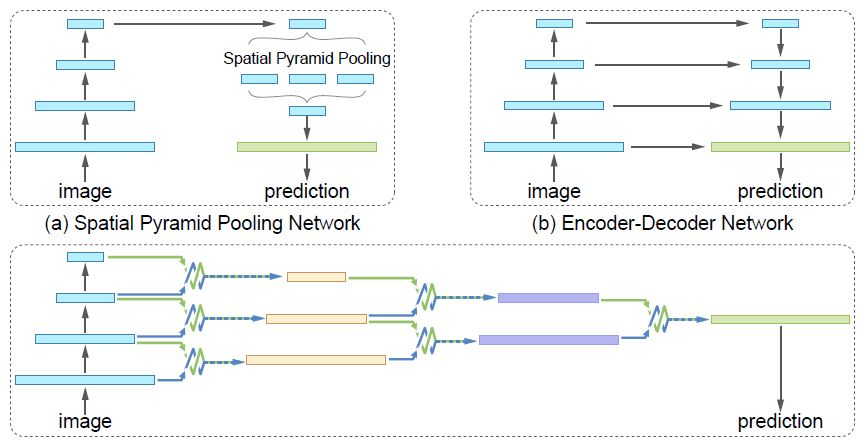
\includegraphics[width=\columnwidth]{fw}
				%		 Create a subtitle for the figure.
			\caption{Multi-Scale context interwining network.}
			\label{fig:fw}
		    \hspace{0.5cm}
			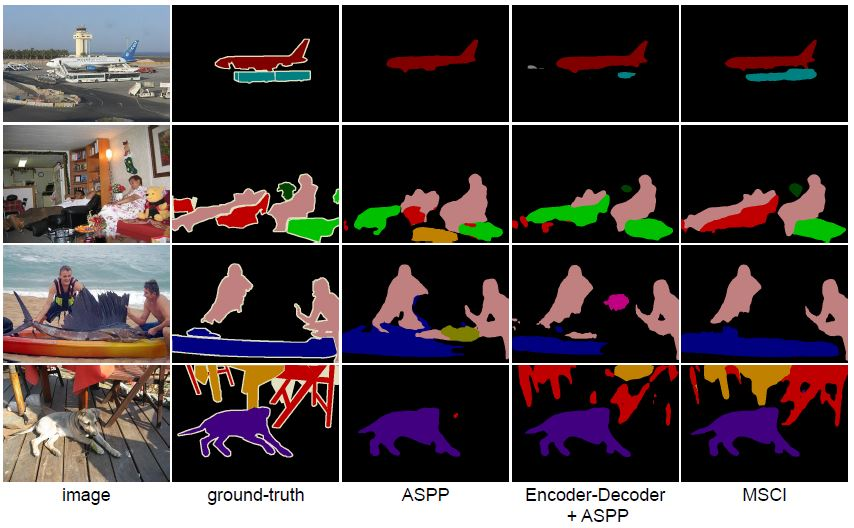
\includegraphics[width=\columnwidth]{rs}
				%Create a subtitle for the figure.
			\caption{Segmentation results of MSCI and other SOTA models.}
			\label{fig:rt}
		\end{center}
	\end{figure}

% Now we need a bibliography:
%\begin{thebibliography}{5}
%
%	%Each item starts with a \bibitem{reference} command and the details thereafter.
%	\bibitem{HOP96} % Transaction paper
%	J.~Hagenauer, E.~Offer, and L.~Papke. Iterative decoding of binary block
%	and convolutional codes. {\em IEEE Trans. Inform. Theory},
%	vol.~42, no.~2, pp.~429–-445, Mar. 1996.
%
%	\bibitem{MJH06} % Conference paper
%	T.~Mayer, H.~Jenkac, and J.~Hagenauer. Turbo base-station cooperation for intercell interference cancellation. {\em IEEE Int. Conf. Commun. (ICC)}, Istanbul, Turkey, pp.~356--361, June 2006.
%
%	\bibitem{Proakis} % Book
%	J.~G.~Proakis. {\em Digital Communications}. McGraw-Hill Book Co.,
%	New York, USA, 3rd edition, 1995.
%
%	\bibitem{talk} % Web document
%	F.~R.~Kschischang. Giving a talk: Guidelines for the Preparation and Presentation of Technical Seminars.
%	\url{http://www.comm.toronto.edu/frank/guide/guide.pdf}.
%
%	\bibitem{5}
%	IEEE Transactions \LaTeX and Microsoft Word Style Files.
%	\url{http://www.ieee.org/web/publications/authors/transjnl/index.html}
%
%\end{thebibliography}

% Your document ends here!
\end{document}